\subsection{Pulssensorer}\label{sec:pulssensor}
Kroppens puls kan detekteres på en række forskellige måder, eksempelvis elektrisk eller optisk.
Elektriske pulssensorer, måler pulsen ved hjælp af en elektrisk kontaktflade mellem sensor og person, hvilket skabes ved hjælp af elektroder. Pulsen detekteres af de elektriske pulssensorer, som forskelle i den elektriske ladning. Udfaldet af målingerne kan være afvigende, da individuelle faktorer såsom en personens blod, svedniveau eller hudfedt er en afgørende faktor. For at minimere disse udfald kræves der en god elektronisk kontakt, heraf er præparering af huden nødvendig. Denne type plusmåling kræver en placering ved hjertets afledninger\fxnote{Kig her for at se hjertets afledninger: https://www.sundhed.dk/borger/sygdomme-a-aa/hjerte-og-blodkar/illustrationer/tegning/placering-af-ekg-elektroder/}. \citep{PhuaLissorguesMercier2009}  \\
Optiske pulssensorer registrerer puls ved hjælp af lysindhold. En LED udsender en lyskilde som passerer huden og en blodåre, hvoraf en mængde af dette lys absorberes af hæmoglobin i blodet. Efterfulgt af dette opfanger en fotodiode mængden af det resterende lys. Størrelsen af dette lys er den bestemmende faktor vedrørende mængde af blod i blodåren, og er heraf omvendt proportionalt. Pulssensoreren udsender positive udsalg på signalet, desto mere blod der registreres. Denne type sensor placeres derfor over en blodåre.\citep{PhuaLissorguesMercier2009,SrinivasReddySrinivas2006} 

%\subsubsection{Registrering af puls}
%Pulsen er angivet som forskellen i det systoliske og diastoliske blodtryk som slag per minut. Pulsen kan måles manuelt ved at placere to fingre over en arterie, og derefter tælle hvor mange slag der er i minuttet. Hyppigst måles pulsen fra radial arterien på håndleddet eller på halsen, men enhver arterie der kan mærkes, kan bruges til at måle pulsen ved, se \figref{pulsmaaling}. \citep{CNX2016}
%
%\begin{figure}[H]
%	\centering
%	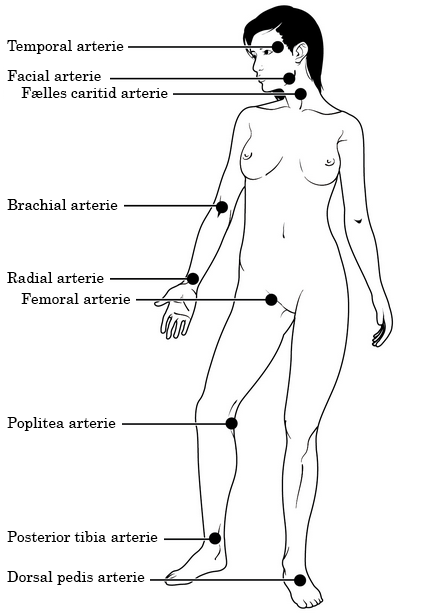
\includegraphics[scale=0.6]{figures/bProblemloesning/puls.png}
%	\caption{På figuren ses steder det er muligt at måle puls.\citep{CNX2016}}
%	\label{fig:sensor_placering}
%	\end{figure}
	


